\chapter{Nozioni introduttive}
Viviamo in un era digitale, le immagini passano generalmente per un calcolatore prima di essere stampate, o in ogni caso possono essere sempre scannerizzate (con strumenti più o meno precisi) così da averne una copia digitale.
E' in questa fase che l'immagine subisce il processo di filtraggio, nel calcolatore, quando pè in formato digitale, Per capire cos'è un filtro occorre dunque chiedersi cosa sia un'immagine digitale.

\section{Immagini digitali}
Per capire come codificare un'immagine per memorizzarla in fgormato digitale ci chiediamo prima che cos'è un'immagine.

\begin{quote}
\epigraph{Forma esteriore degli oggetti corporei, in quanto viene percepita attraverso il senso della vista, o si riflette – come realmente è, o variamente alterata – in uno specchio, nell’acqua e sim., o rimane impressa in una lastra o pellicola o carta fotografica.}{Vocabolario Treccani}
\end{quote}


\noindent
Un'immagine viene rappresentata, impressa quindi su superfici, cioè oggetti bidimensionali, di dimensioni finite e le vediamo perchè i nostri occhi percepiscono il susseguirsi di colori diversi. Come codificare tali entità?
Come tutti gli oggetti reali, sebbene abbiano dimensioni finite, il susseguirsi delle immagini avviene in una maniera che possiamo considerare come continua. Questo è il primo problema che ci si pone quando si pensa a come codificare delle immagini.
La soluzione più largamente utilizzata è anche quella più semplice ed intuitiva, ossia di discretizzare tale distribuzione di colori. Dividiamo l'immagine con una griglia ed ad ogni casella, che d'ora in poi chiameremo "pixel", assegnamo un colore. 
E' ovvio che così facendo si perdono dei dettagli, la quantità di dettagli che riusciamo a conservare piò variare enormemente, un minimo si perde sempre ma è un prezzo che siamo disposti a pagare.\\
Facciamo un esempio:

%\ref{fig:figuraa}. 
\begin{figure}[htb] \centering
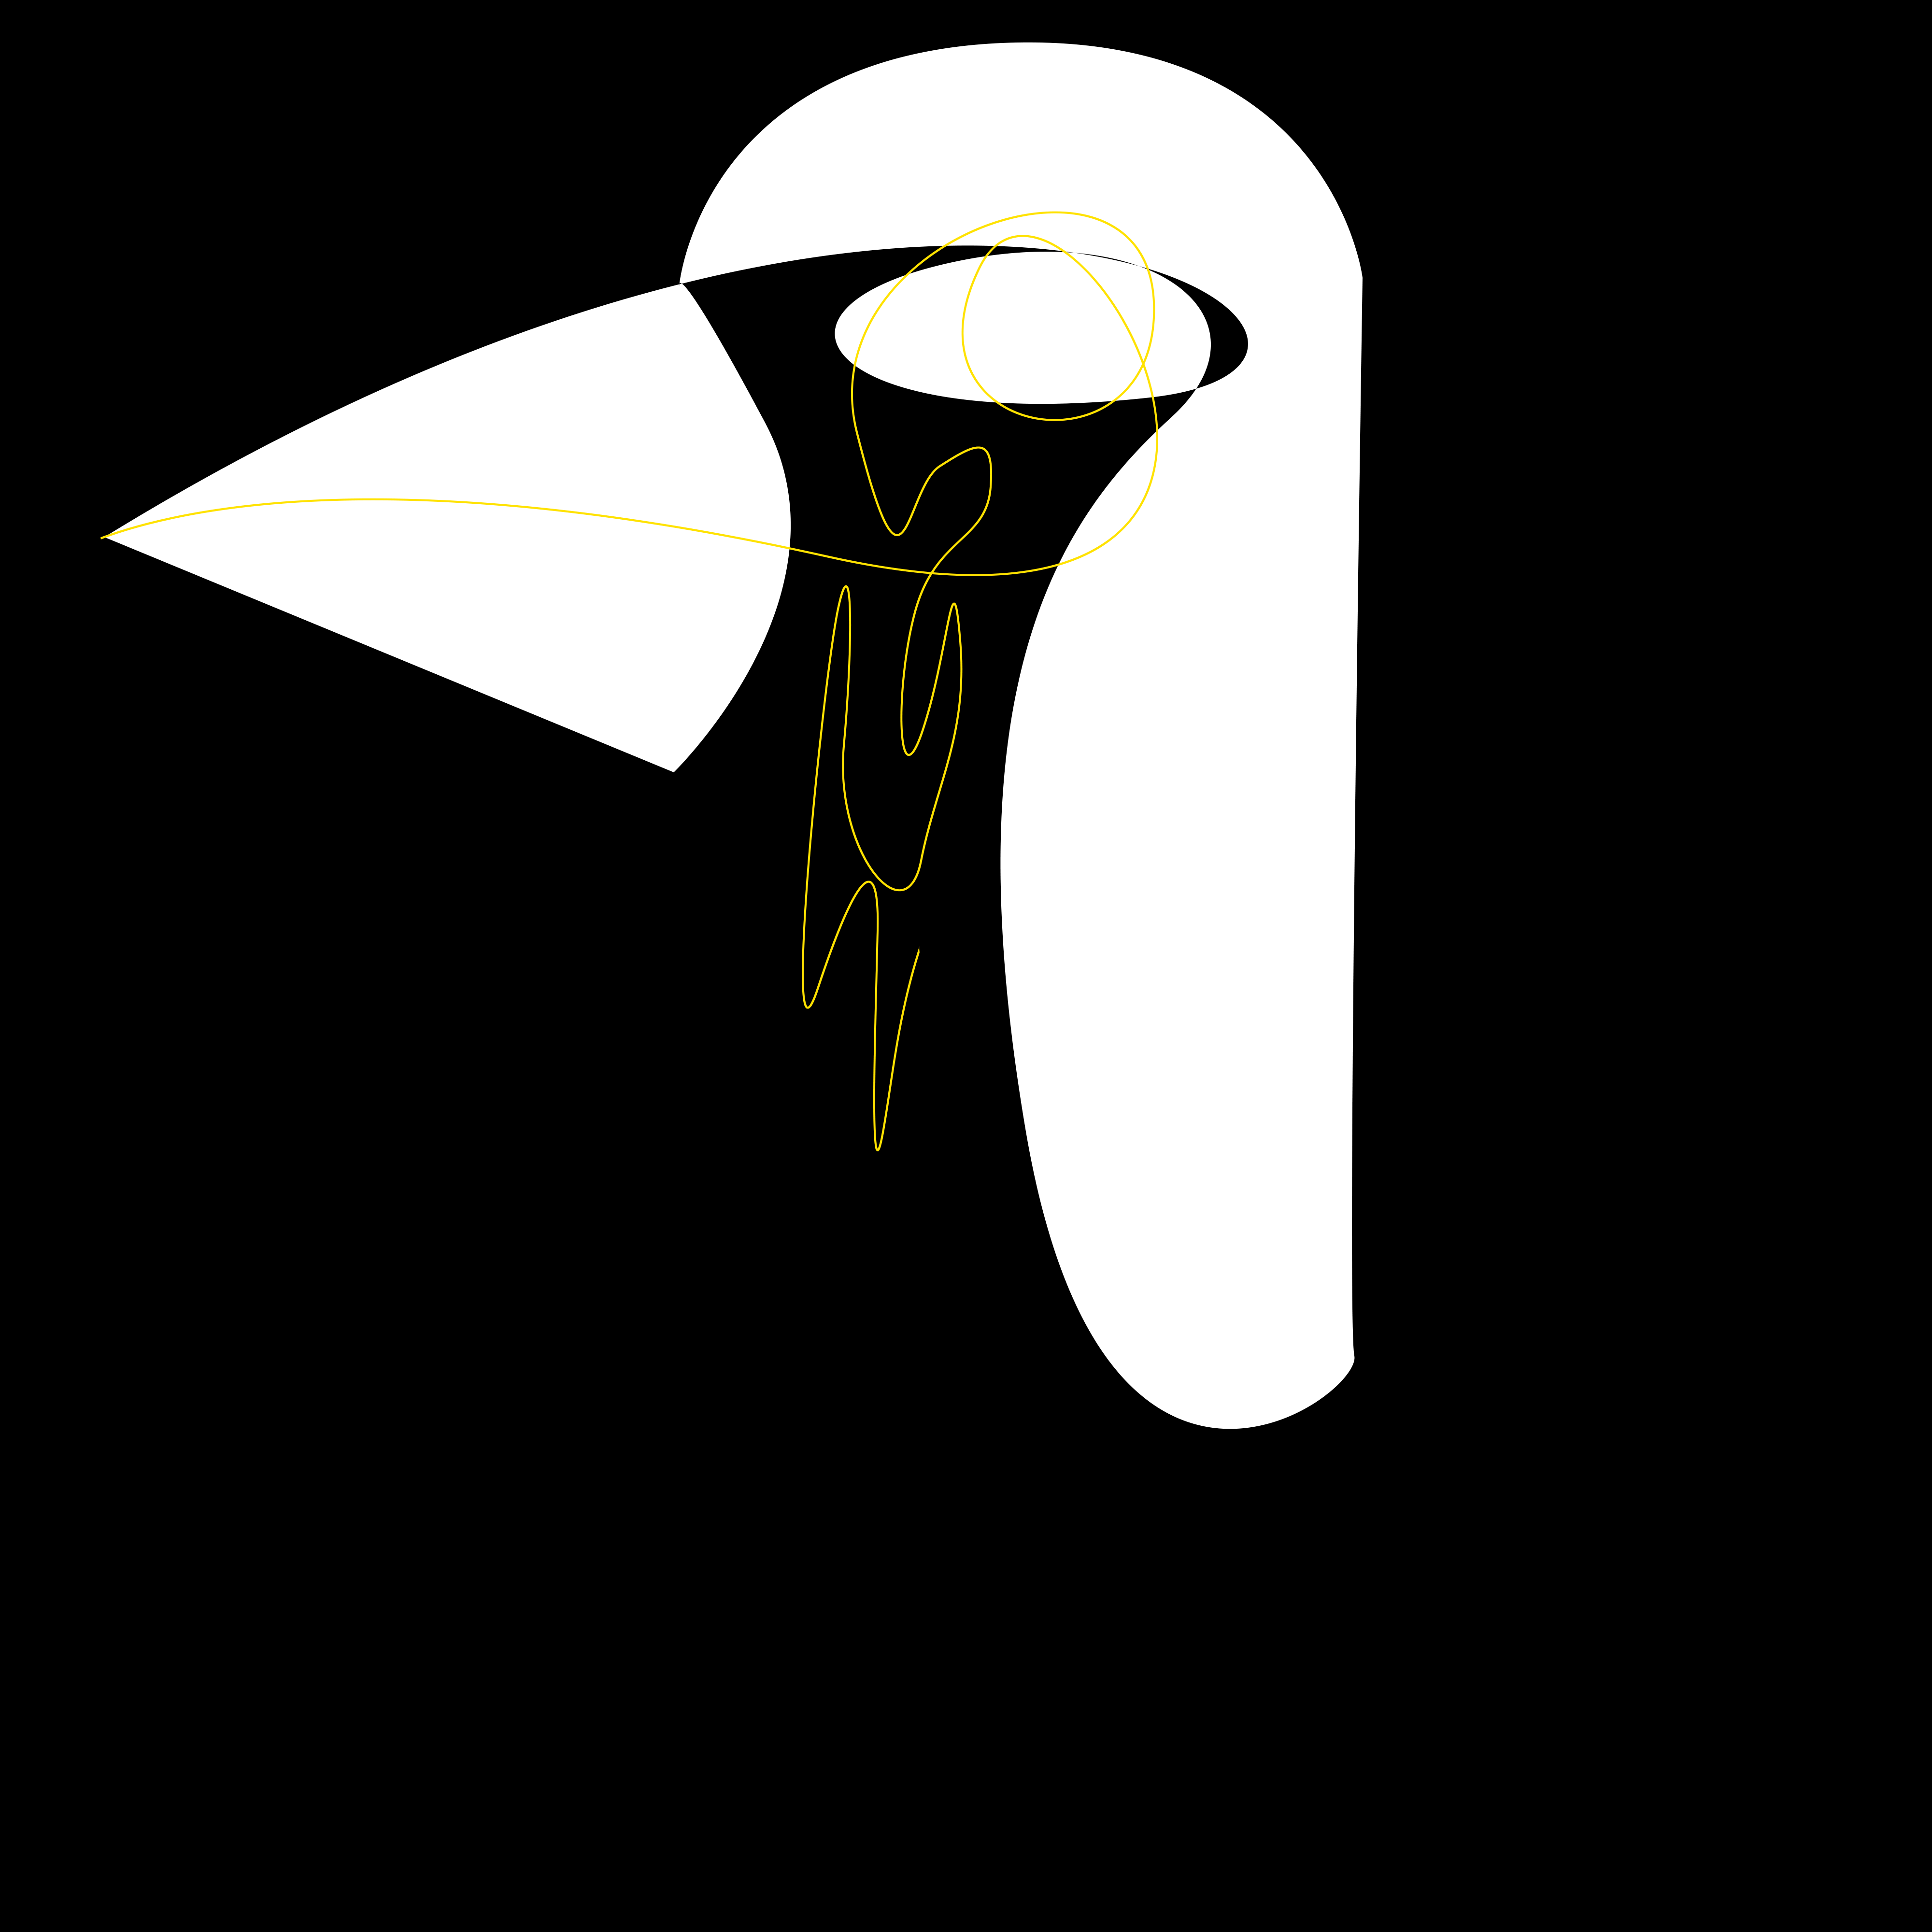
\includegraphics[scale=0.03]{Pictures/in ricordo del pinguino cameriere.png}
%\caption{Fiamme.}\label{fig:figura}
\qquad\qquad

\includegraphics[scale=0.03]{Pictures/canvas8x8.png}
\caption{Confronto immagine originale e immagine codificate utilizzando una griglia 4x4.}\label{fig:figura}
\end{figure}

%\ref{fig:figura}. 
\begin{figure}[htb] \centering
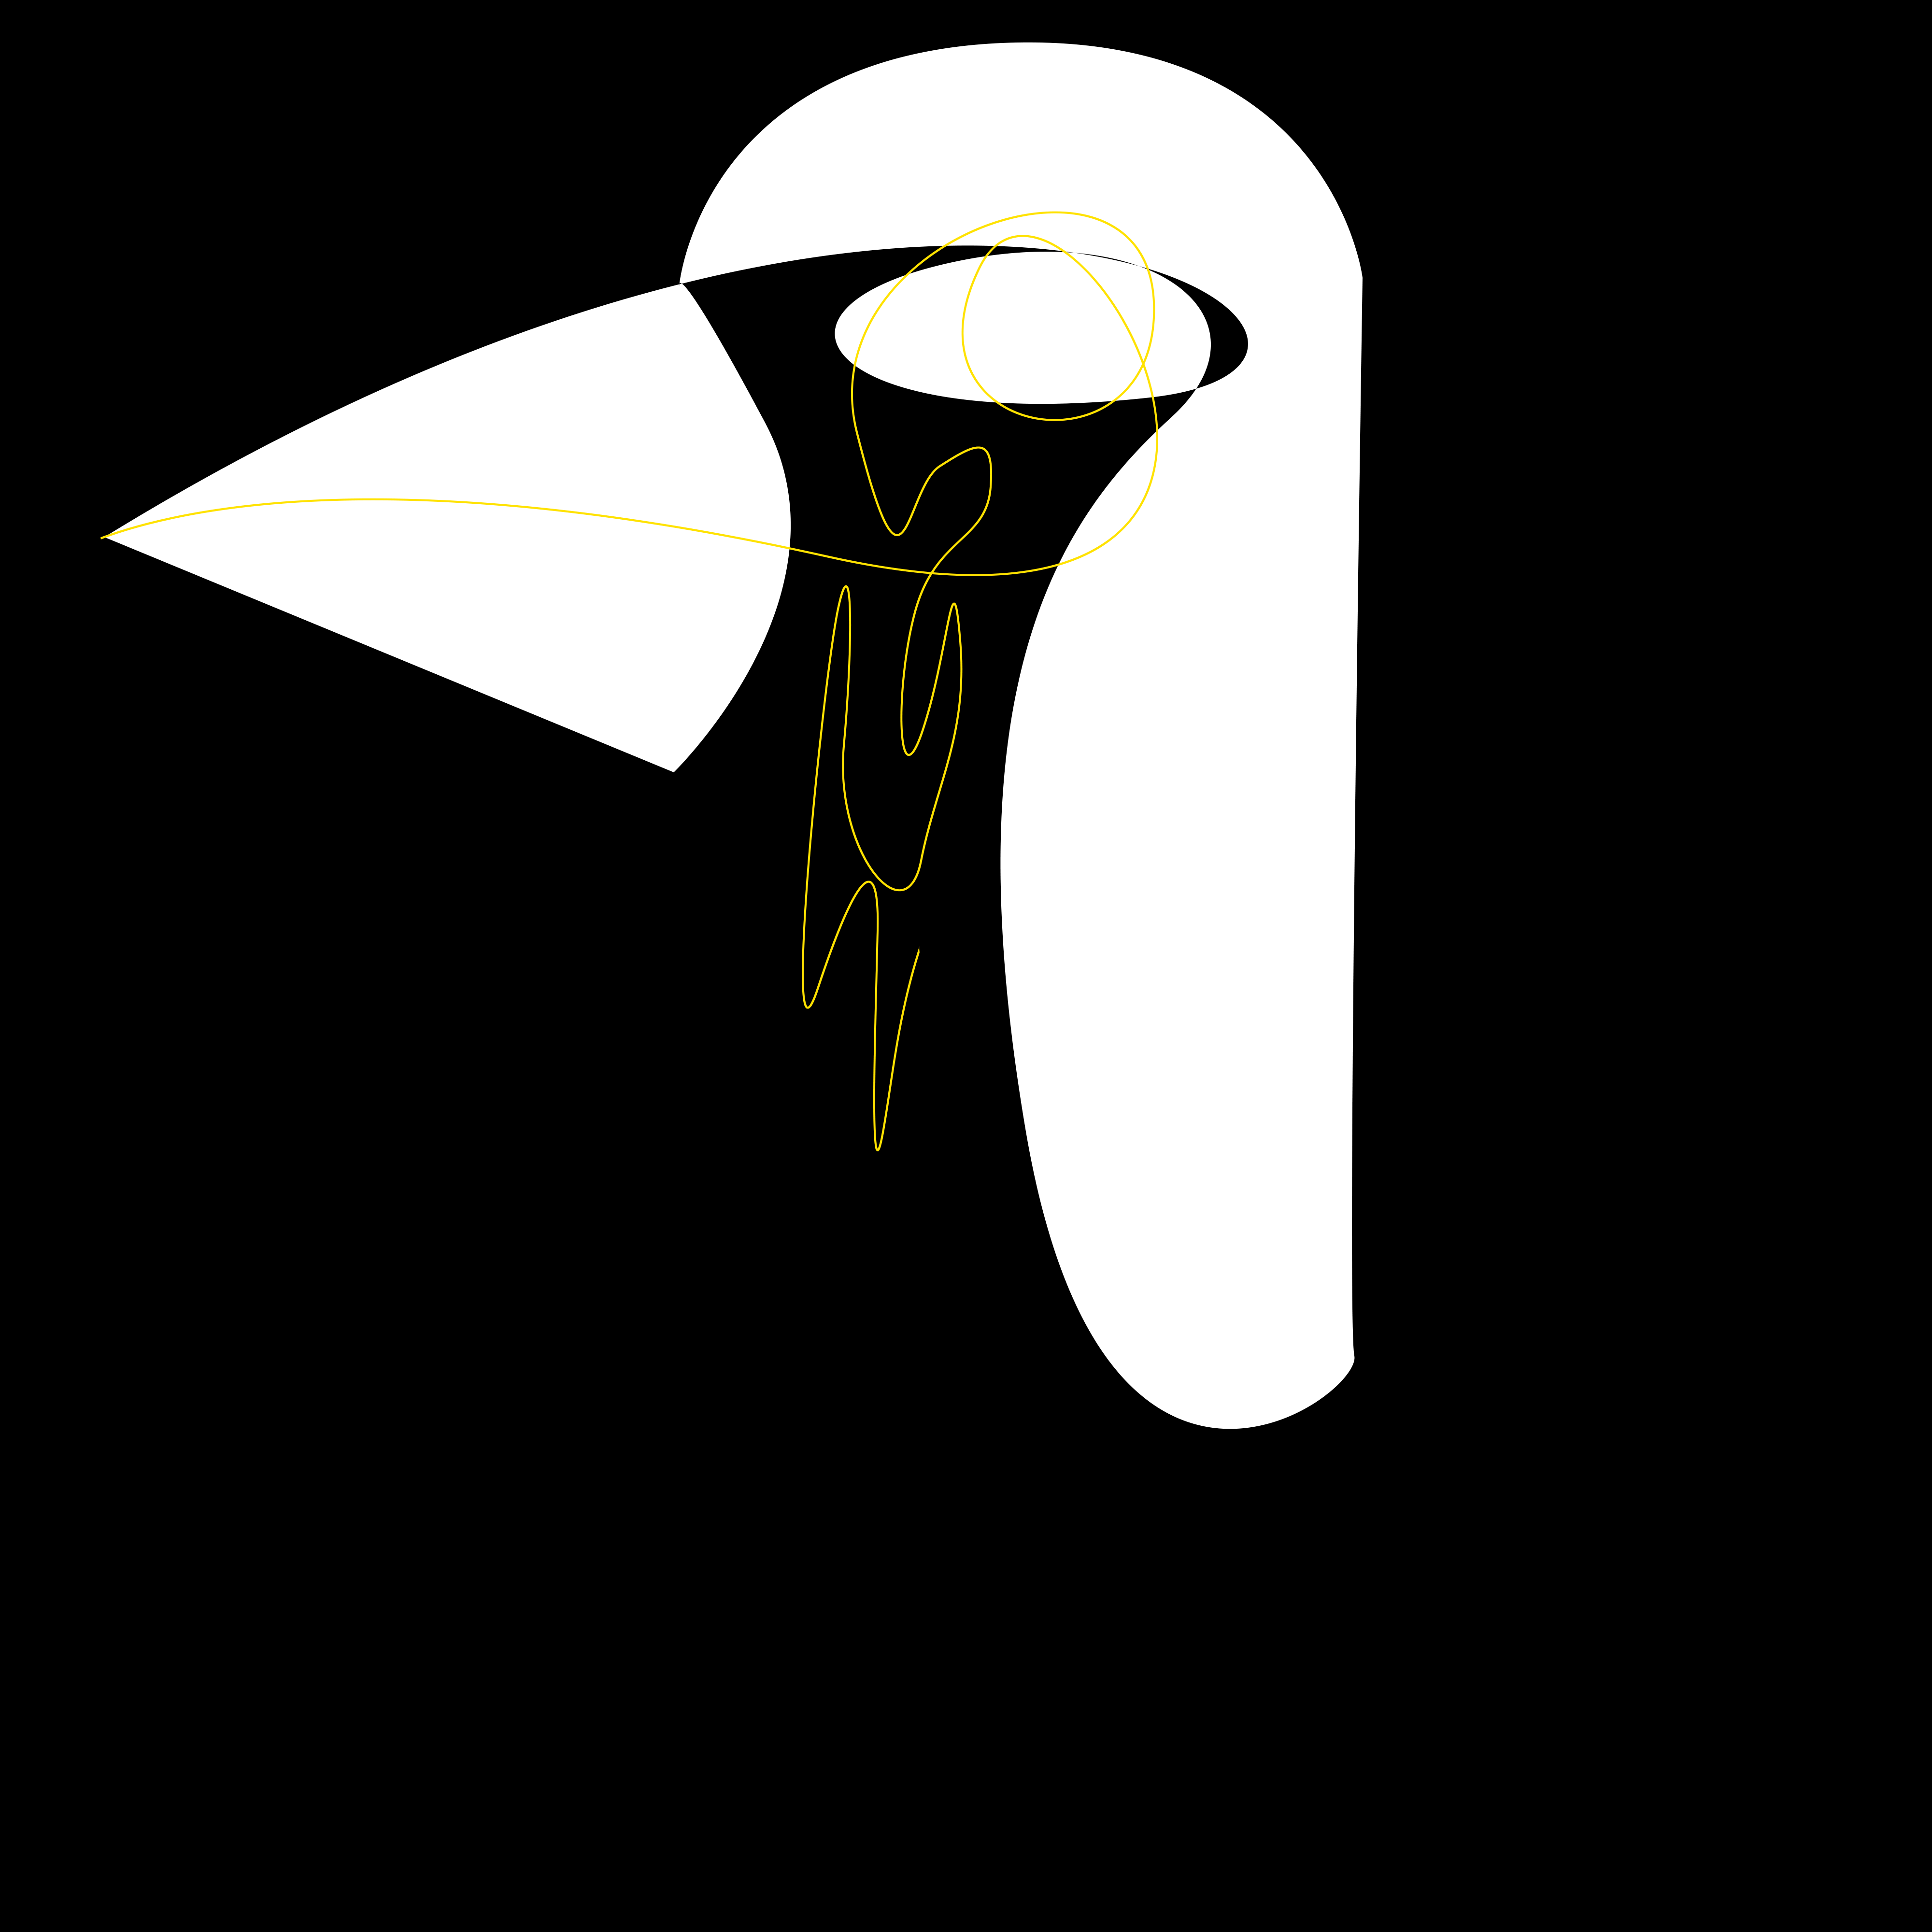
\includegraphics[scale=0.03]{Pictures/in ricordo del pinguino cameriere.png}
%\caption{Fiamme.}\label{fig:figura}
\qquad\qquad
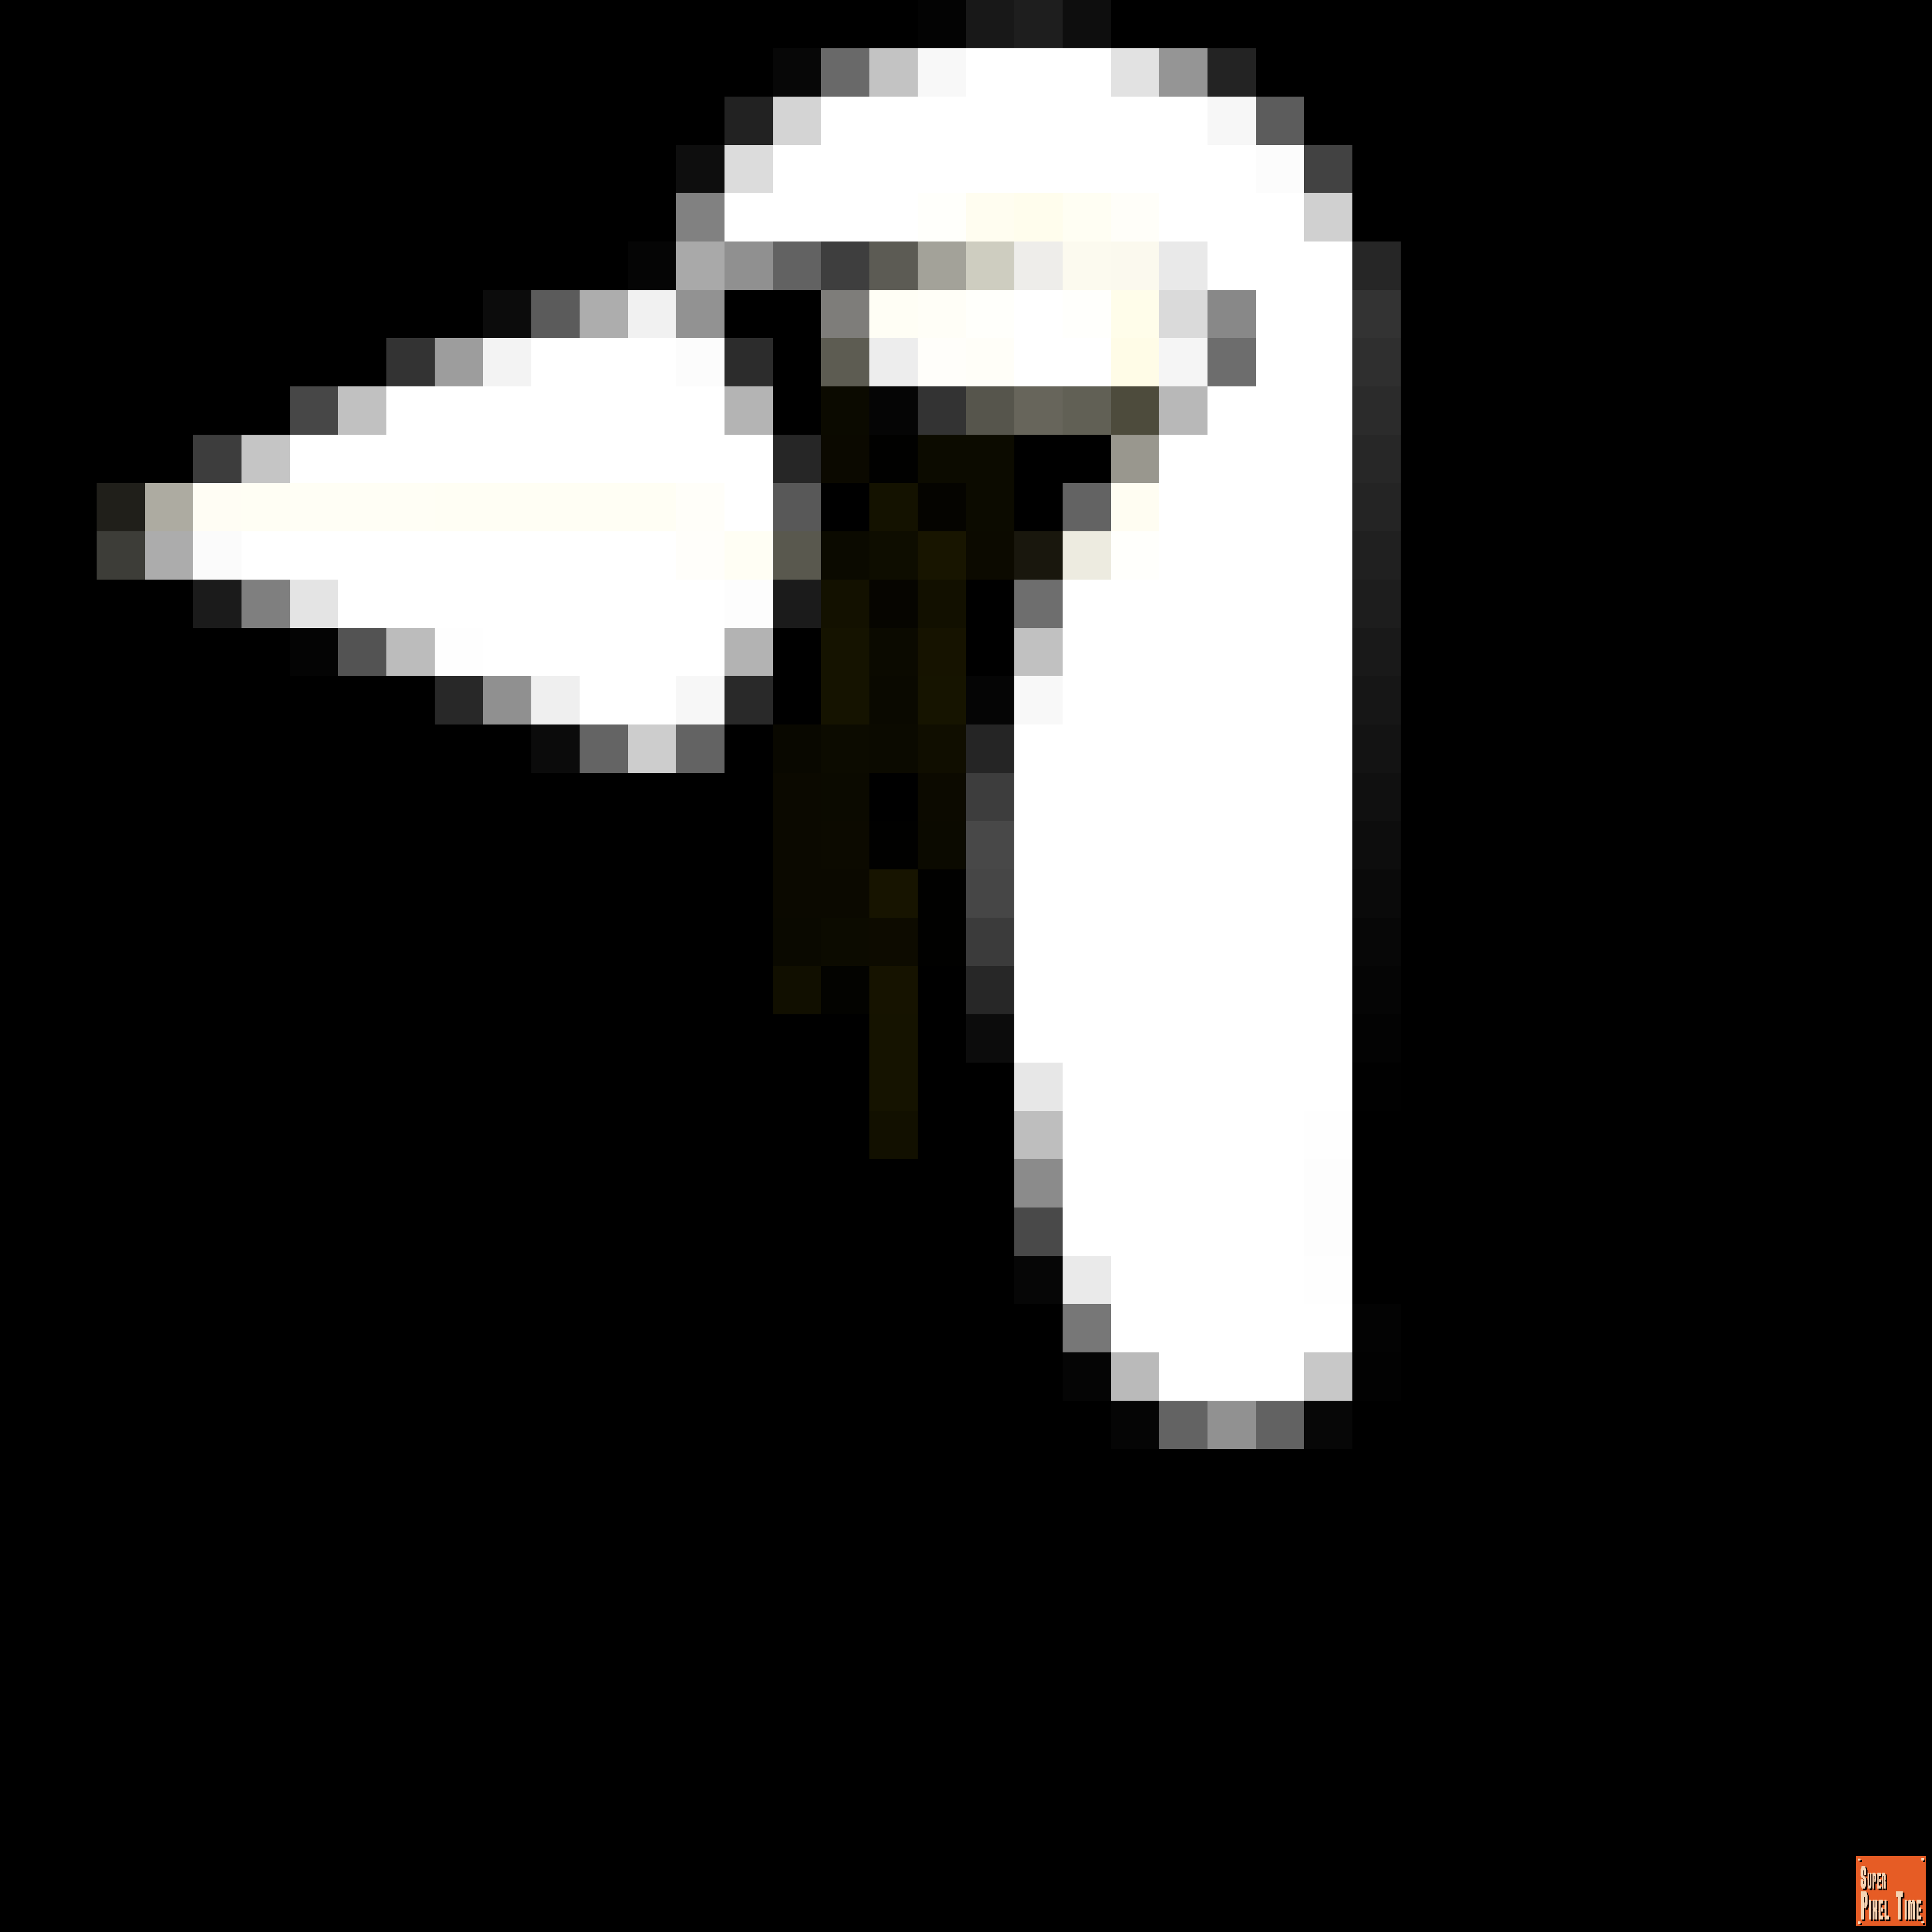
\includegraphics[scale=0.03]{Pictures/canvas80x80.png}
\caption{Confronto immagine originale e immagine codificate utilizzando una griglia 80x80.}\label{fig:figura}
\end{figure}

\noindent
E' semplice vedere come ad una griglia più fitta corrisponda una miglior qualità dell'immagine, questo è il concetto di "risoluzione di un'immagine". 
Una miglior risoluzione però costa, come anticipato, in termini di memoria. Una griglia 4x4 corrisponde a 16 pixel, ad una griglia 80x80 corrispondono invece 6400 pixel! Questo vuol dire che la seconda immagine pesa 400 volte di più della prima.

\vspace{1em} \noindent
Volendo definire in maniera più precisa cosa e' un'immagine digitale, diremmo che quest'ultima è una funzione da $\mathbb R^2$ in $\mathbb R^3$ cioè, date in input due coordinate, essa restituisce un colore (che è formato da 3 canali RGB). Se però l'immagine è in bianco e nero la questione si semplifica: l'immagine diventa una funzione da $\mathbb R^2$ in $\mathbb R$, dal momento che per codificare un colore appartenente alla scala di grigio basta un solo canale, il livello di luminosità. Difatti, la riduzione da tre ad un solo canale rappresenta un grosso vantaggio, permettendo di diminuire di due terzi lo spazio di memoria occupato.

\section{Cosa sono i filtri}
Una volta capito che un'immagine è una funzione possiamo definire un filtro come una seconda funzione che convoluta alla prima da il risultato richiesto.

\noindent
Una equazione alle derivate parziali (PDE) esprime una evoluzione, sia u la nostra immagine e $u_0$ lo stato in cui si trova inzialmente, allora per convoluzione possiamo dire che 

\begin{equation} \label{eq:eq3}
u(x)=\frac{1}{w(x)}\int\int d(x-\xi)\Tilde{d}(u_0(x) -u_0(\xi))u_0(\xi)d\xi.
\end{equation}

\centering con  $w(x) = \int\int d(x-\xi)\Tilde{d}(u_0(x) -u_0(\xi))d\xi$\newline

\raggedright

Definiti questi concetti siamo pronti ad iniziare la trattazione vera e propria

